%%%% Document type  %%%%
%\documentclass[preprint,12pt,fleqn]{article}
\pdfoutput=1
\documentclass[12pt]{article}
\usepackage{ragged2e}
\usepackage{graphicx}

% \usepackage{nopageno} % no page numbers
\usepackage{placeins} % \FloatBarrier
\usepackage{upgreek, bm}

\usepackage[most]{tcolorbox}
\newtcolorbox[auto counter,number within=chapter]{definition}[1][]{
  enhanced,
  breakable,
  fonttitle=\scshape,
  title={Definition \thetcbcounter},
  #1
}

%%%% Document structure %%%%
%\usepackage{geometry}
\usepackage[verbose=true,letterpaper]{geometry}
\geometry{
    textheight=9in,
    textwidth=6in,
    top=1in,
    headheight=12pt,
    headsep=25pt,
    footskip=30pt,
}

\usepackage{lineno} % used along with \linenumbers after begin document. 
\usepackage{setspace} 
\setstretch{1.25}
\makeatletter % The following lines get rid of footer stating pre-preint to elsevier.
\def\ps@pprintTitle{%
\let\@oddhead\@empty
\let\@evenhead\@empty
\def\@oddfoot{}%
\let\@evenfoot\@oddfoot}
\makeatother
\graphicspath{ {../images/} }
\usepackage{pgf} % calculate cohort stats percentage

%%%% Bibliography   %%%%
\usepackage{natbib}
\setcitestyle{numbers,sort&compress}
\setcitestyle{sort&compress}
\usepackage{hypernat} 
    
%%%% Aesthetics     %%%%
\usepackage{microtype}
% \RequirePackage{times} % Font
\usepackage{ccaption}
\usepackage{siunitx}
\usepackage[T1]{fontenc}
\usepackage[utf8]{inputenc}
\usepackage{nameref}% this allows a reference be named, to print unnumbered references by their section name (used here for linking to Supplemental text in this case).

%%%% Paragraph Formatting %%%
% \setlength{\parindent}{0pt}
\setlength{\parindent}{15pt}
\setlength{\parskip}{6pt plus 2pt minus 1pt}

%%%% Supplemental labels%%%%
%Define command to start a supplemental section
%set the supplemental letter used for figures (e.g. Figure E1)
\newcommand{\beginsupplement}{%
        \setcounter{table}{0}
        \renewcommand{\thetable}{S\arabic{table}}%
        \setcounter{figure}{0}
        \renewcommand{\thefigure}{S\arabic{figure}}%
         }

%%%% Building tables%%%%
\usepackage{booktabs} % required for tables
\usepackage{rotating,tabularx} 
\newcolumntype{Z}{ >{\centering\arraybackslash}X } % defining table content layout per box
\usepackage{ltablex} % allow page break between lines in tabularx
% \usepackage{caption} \captionsetup{font=normalsize} % to set the caption size as normal even when table is tiny.
\usepackage{multirow}
\usepackage{pdflscape}

%%%% Colors %%%%
\usepackage{xcolor} 
\definecolor{natureblue}{RGB}{5,110,210}
    \usepackage[colorlinks]{hyperref} 
\AtBeginDocument{%this allows colours to chage from the defined elsearticle template.
\hypersetup{
    	colorlinks=true,
        linkcolor={natureblue},
    	citecolor={natureblue},
        filecolor=blue!50!black,
        urlcolor=cyan,
    	}}

\definecolor{kispiblack}{HTML}{333333}
\definecolor{kispidarkblue}{HTML}{023047}
\definecolor{kispidarkgreen}{HTML}{006666}
\definecolor{kispired}{HTML}{C70000}
\definecolor{kispilink}{HTML}{007DB8}%219EBC
% \color{kispi_black} %default
\definecolor{kispiblue}{HTML}{701A57}
% City sunset: https://www.color-hex.com/color-palette/40131
\definecolor{colorSUNSET1}{HTML}{eeaf61}
\definecolor{colorSUNSET2}{HTML}{fb9062}
\definecolor{colorSUNSET3}{HTML}{ee5d6c}
\definecolor{colorSUNSET4}{HTML}{ce4993}
\definecolor{colorSUNSET5}{HTML}{6a0d83}
\definecolor{natureblue}{RGB}{5,110,210}    
\usepackage{dirtree}  % Load the dirtree package

% command to use these colors and formatting; xspace for correct spacing including with punctuation marks.
\usepackage{xspace}
\newcommand{\variablesdarkgreen}[1]{\textbf{\textcolor{kispidarkgreen}{#1}}\xspace}
 
\usepackage{tocloft}  % Customizing the Table of Contents
\setcounter{tocdepth}{2}

%%%% Include code %%%%
% \usepackage{verbatim}
\usepackage{listings}
\lstset{
    basicstyle=\ttfamily\small,
    breaklines=true,
    postbreak=\mbox{\textcolor{red}{$\hookrightarrow$}\space}, % 
    breakatwhitespace=false,
    % frame=single,
    showstringspaces=TRUE, % Don't show spaces in strings as special characters
    tabsize=2, 
    language=sh 
}

\usepackage[printonlyused,withpage,nohyperlinks]{acronym}
\usepackage{tikz}
\usetikzlibrary{calc}
\usepackage{amsmath, amssymb}

% author affil
\usepackage{authblk}
\renewcommand\Authfont{\normalsize}
\renewcommand\Affilfont{\small}
\setlength{\affilsep}{1em}

\begin{document}

\newcounter{myboxcounter}
\newcommand{\boxlabel}[1]{%
  \refstepcounter{myboxcounter}%
  \label{#1}%
}

\title{Quantifying prior probabilities for disease-causing variants reveals the top genetic contributors in inborn errors of immunity}

% in your preamble, before \author:
\newcommand{\QUANT}{1}
\newcommand{\GHI}{2}
\newcommand{\KISPIIMM}{3}
 \newcommand{\METAB}{4}
\newcommand{\LEEDS}{5}
\newcommand{\IPSNEO}{6}

\author[\QUANT]{Quant Group} 
\author[\GHI]{Simon Boutry}% \textsuperscript{†}}
\author[\GHI]{Ali Saadat}% \textsuperscript{†}} \textsuperscript{†}}
\author[\KISPIIMM]{Maarja Soomann}% \textsuperscript{†}} \textsuperscript{†}}
\author[\KISPIIMM]{Johannes Trück}
 \author[\METAB]{D. Sean Froese}
\author[\GHI]{Jacques Fellay}
\author[\LEEDS]{Sinisa Savic}% orcid.org/0000-0001-7910-0554
\author[\IPSNEO]{Luregn J. Schlapbach}
\author[\IPSNEO]{Dylan Lawless *%\thanks{Addresses for correspondence: \href{mailto:Dylan.Lawless@kispi.uzh.ch}{Dylan.Lawless@kispi.uzh.ch}}
}
% \textsuperscript{†}
\affil[\QUANT]{The quantitative omic epidemiology group.} 
\affil[\GHI]{Global Health Institute, School of Life Sciences, École Polytechnique Fédérale de Lausanne, Switzerland.}
\affil[\KISPIIMM]{Division of Immunology and the Children’s Research Center, University Children’s Hospital Zurich, University of Zurich, Zurich, Switzerland.}
 \affil[\METAB]{Division of Metabolism and Children’s Research Center, University Children’s Hospital Zürich, University of Zurich, Zurich, Switzerland.}
\affil[\LEEDS]{Leeds Institute of Rheumatic and Musculoskeletal Medicine, University of Leeds, Leeds, UK.}
\affil[\IPSNEO]{Department of Intensive Care and Neonatology, University Children's Hospital Zurich, University of Zurich, Zurich, Switzerland.}

\maketitle
\justify

%Abstract: 150 of 150. Main text:  3931 of 4000 (intro, result, discussion, conclusion). Display (4 figures / 2 tables) of 8 total. Extended display: x of 10. Note that this journal uses separate online methods.

\noindent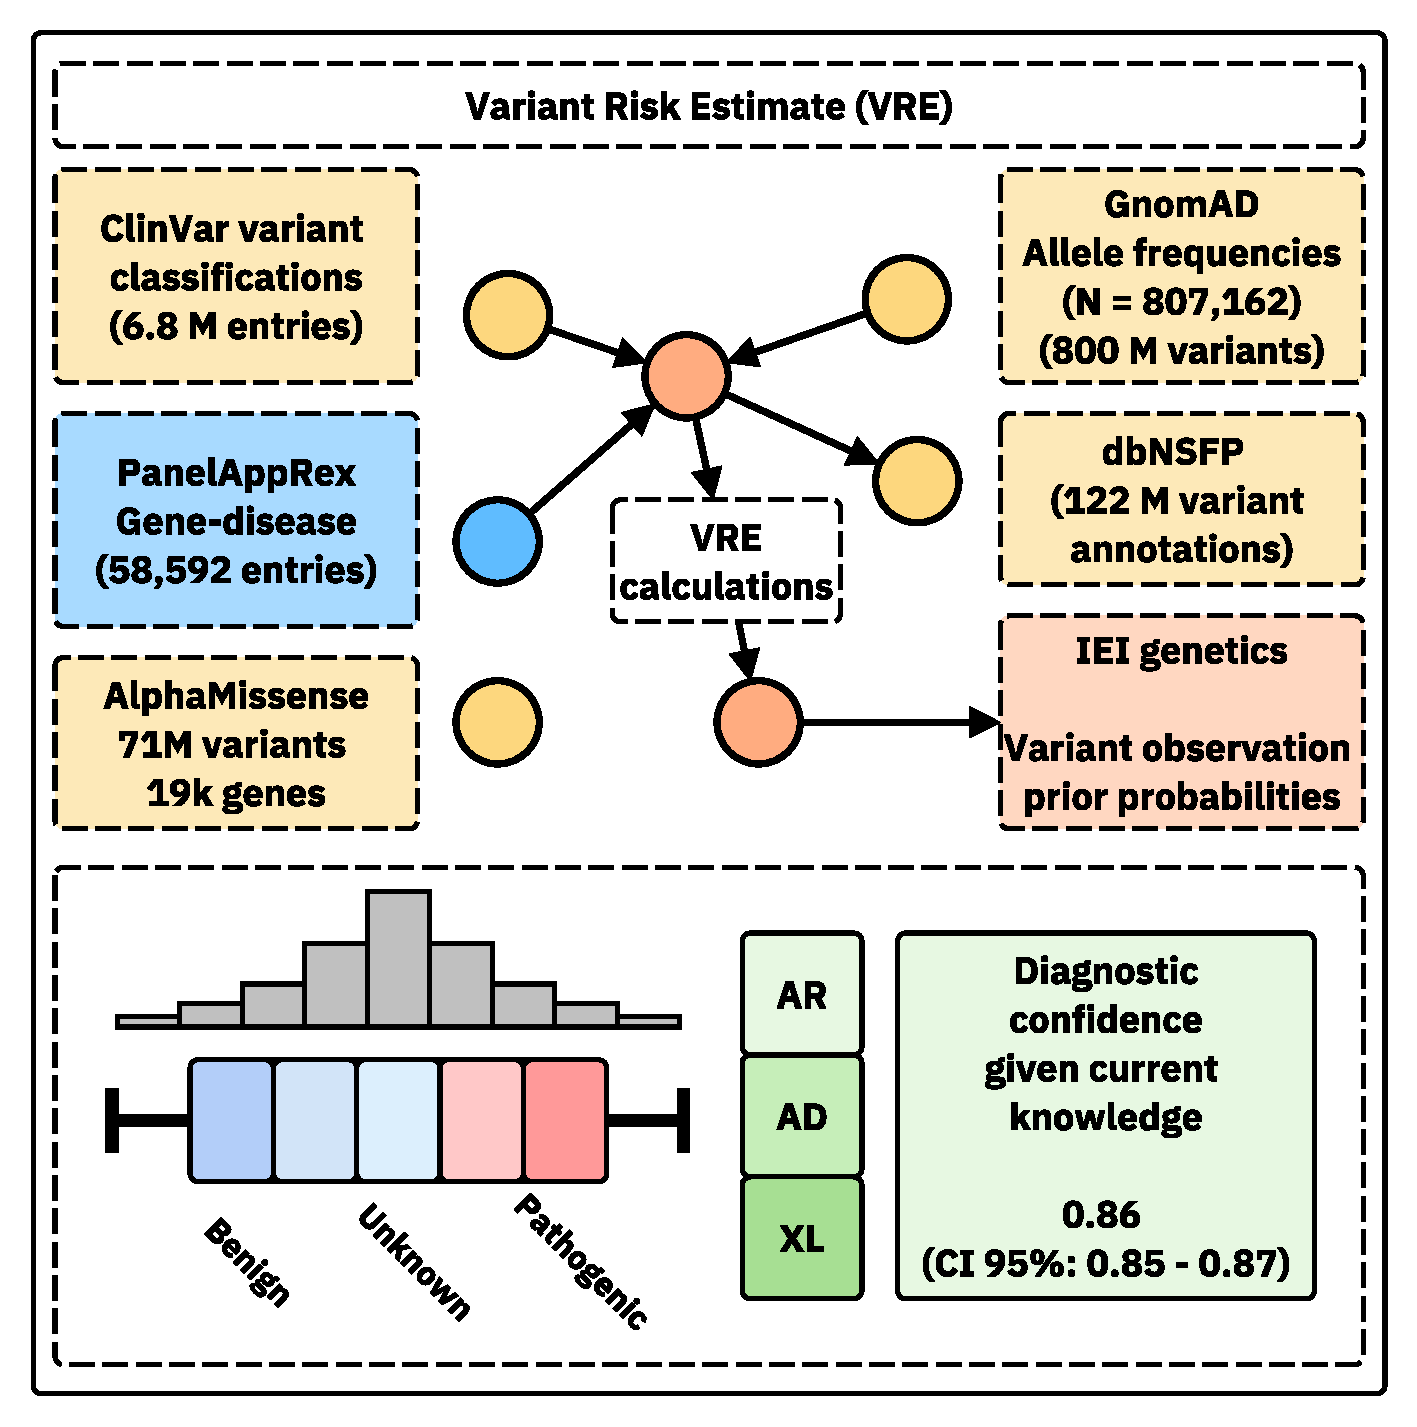
\includegraphics[width=0.7\textwidth]{./images/var_risk_est_ci.pdf}

\noindent Graphical abstract.

\clearpage
%  \linenumbers
\begin{abstract} 

\noindent \textbf{Background}:
Accurate interpretation of genetic variants requires a quantitative estimate of how likely a variant is to contribute to disease, accounting for both observed and unobserved causal alleles across different inheritance modes.
\vspace{1em}

\noindent \textbf{Methods}:
We developed a statistical framework that computes genome-wide prior probabilities for variant classification by integrating population allele frequencies, disease classifications, and Hardy-Weinberg expectations across dominant, recessive, and X-linked inheritance. Bayesian modelling then combines these priors with individual-level data to produce credible intervals that quantify diagnostic confidence.
\vspace{1em}

\noindent \textbf{Results}:
The framework replaces categorical variant classification with continuous posterior probabilities that capture residual uncertainty from incomplete or missing genotype data. Demonstrations in three diagnostic scenarios show accurate quantification of variant-level disease relevance. Application to 557 genes implicated in inborn errors of immunity (IEI) generated a public database of prior probabilities. Integration with protein-protein interaction and immunophenotypic data revealed gene-level constraint patterns, and validation in national cohorts showed close agreement between predicted and observed case numbers.
\vspace{1em}

\noindent \textbf{Conclusions}:
Our method addresses a long-standing gap in clinical genomics by quantifying both observed and unobserved genetic evidence in disease diagnosis. It provides a reproducible probabilistic foundation for variant interpretation, clinical decision-making, and large-scale genomic analysis.
\footnote{
\noindent * Addresses for correspondence: \href{mailto:Dylan.Lawless@uzh.ch}{Dylan.Lawless@uzh.ch}.\\
% \noindent  \textsuperscript{† }These authors contributed equally and are listed alphabetically.\\
\textbf{Availability:} This data is integrated in public panels at 
% \url{https://switzerlandomics.ch/services/panelAppRexAi/} and 
\url{https://iei-genetics.github.io}.
The source code are accessible as part of the variant risk estimation project at \url{https://github.com/DylanLawless/var_risk_est} and IEI-genetics project at
\url{https://iei-genetics.github.io}.
The data is available from the Zenodo repository: 
\url{https://doi.org/10.5281/zenodo.15111583}
(VarRiskEst PanelAppRex ID 398 gene variants.tsv).
VarRiskEst is available under the MIT licence.
% \url{https://github.com/TheQuantGroup/QauntGroup}.
}
\vfill
\end{abstract}


\section{Introduction}
Accurately estimating the probability that a patient carries a disease-causing genetic variant remains a central challenge in clinical and statistical genetics. For over a century, attention has focused on identifying variants which are \ac{tp} and reducing \ac{fp}, while \ac{fn} and \ac{tn} have received comparatively little consideration. \ac{fn} arise when pathogenic variants are missed due to technical or interpretive limits, and \ac{tn} represent the vast background of benign variants. Although \ac{tn} have clear value in contexts such as cancer screening, their wider statistical and clinical relevance remains underused. From a probabilistic standpoint, \ac{fn} and \ac{tn} provide crucial information about what is not observed, what should be expected under baseline genetic assumptions, and how confident one can be in the absence of a pathogenic finding. In practice, variant interpretation still relies on deterministic tools. For instance, GATK is used for processing; Ensembl VEP, SnpEff, FAVOR, and WGSA perform variant effect prediction \cite{2024riccioVariantEffectPredictors}; and Exomiser and VarFish support interpretation \cite{2020ciprianiImprovedPhenotypeDrivenTool, 2020holtgreweVarFishComprehensiveDNA}. These tools focus on annotation and prioritisation but don't have access to the underlying probabilities.

Quantifying the risk that a patient inherits a disease-causing variant is a core problem in genomics. Classical approaches based on \ac{hwe} \cite{MayoCentury2008, AbramovsHardyWeinberg2020} have long provided the foundation for calculating variant probabilities. However, these models become more complex when extended to different \ac{moi}, such as \ac{ar}, \ac{ad}, or \ac{xl} disorders. In \ac{ar} diseases, risk depends on both homozygosity and compound heterozygosity, whereas a single allele can cause disease in \ac{ad} or \ac{xl} forms. Modern evidence shows that \ac{moi} can be further modulated by mechanisms including dominant negative effects, haploinsufficiency, mosaicism, and digenic or epistatic interactions \cite{zschocke_mendelian_2023}. Although \citet{karczewski2020mutational} advanced the field considerably, applying statistical genomics data across all \ac{moi} for any gene-disease combination remains unresolved. Recent disease-specific estimates, including Wilson disease, mucopolysaccharidoses, primary ciliary dyskinesia, and treatable metabolic disorders \cite{bick_estimating_2025, evans_estimating_2021}, as reviewed by \citet{hannah_using_2024}, demonstrate progress but remain limited in scope.

All existing approaches remain limited to single \ac{moi}, specific disorders, or narrow gene sets. An integrated model is needed to unify these perspectives and generate probabilities that can serve as informative priors in a Bayesian framework for variant and disease probability estimation. Such a framework extends classical \ac{hwe}-based methods, strengthens clinical interpretation by clarifying expected genetic outcomes, and enhances analytical models used in statistical genomics.

The resulting dataset from these necessary calculations also holds value for AI and reinforcement learning applications, providing an enriched version of the data underpinning frameworks such as AlphaFold \cite{jumper_highly_2021} and AlphaMissense \cite{cheng_accurate_2023}.

This gap has persisted largely due to the historical absence of harmonised reference datasets. Only recently have resources become available to enable rigorous genome-wide probability estimation, including population allele frequencies (gnomAD v4 \cite{karczewski2020mutational}), curated variant classifications (ClinVar \cite{landrum_clinvar_2018}), functional annotations (UniProt \cite{the_uniprot_consortium_uniprot_2025}), and pathogenicity prediction models (AlphaMissense \cite{cheng_accurate_2023}). We previously introduced PanelAppRex to integrate gene panel data from sources such as \ac{ge} PanelApp, ClinVar, and \ac{uniprot}, enabling structured, machine-readable datasets for variant discovery and interpretation \cite{lawless_panelapprex_2025, martin_panelapp_2019, landrum_clinvar_2018, the_uniprot_consortium_uniprot_2025}. Together, these advances now allow systematic modelling of the expected distribution of variant types, frequencies, and classifications across the genome.

In this study, we report genome-wide probabilities of disease observation across gene-disease combinations, focusing on known \ac{iei} genes, also referred to as \ac{pid} or monogenic inflammatory bowel disease genes \cite{poli_human_2025, lawless_panelapprex_2025, martin_panelapp_2019}. This well-defined genotype-phenotype set, comprising more than 500 gene-disease associations, provides a robust validation of clinical relevance. The latest \ac{iuis} classification and diagnostic guidelines \cite{poli_human_2025, bousfiha_2024_2025} serve as the benchmark reference. We hypothesised that by integrating curated annotations on population \ac{af}, disease phenotypes, \ac{moi} patterns, and variant classifications with \ac{hwe}-based calculations, it would be possible to estimate expected probabilities of disease-associated variants and derive quantitative confidence in genetic diagnosis using these priors.


\section{Results}

\subsection{Quantifying variant probabilities improves classification of inborn errors of immunity}

\subsubsection*{Genes with high pathogenic variant burden show structured network constraint}

%\subsubsection*{Genetic constraint in high-impact protein networks}
We applied the framework to \ac{iei}, a disease area 
% in which we have expertise and
which offers a well-curated gene set to validate genome-wide estimates and demonstrate potential applications \cite{poli_human_2025}. Because pathogenicity in \ac{iei} often reflects shared molecular pathways, we integrated ClinVar-derived variant probabilities with \ac{ppi} data to quantify per-gene pathogenic burden and assess whether constraint clusters within specific networks, consistent with known \ac{iei} categories and immunophenotypes \cite{szklarczyk2025string, karczewski2020mutational}.

%\subsubsection*{Score-positive-total reveals genes with the highest pathogenic variant burden}
ClinVar classifications (\textbf{Figure \ref{fig:p_varRisEst_summary_scores}}) were scaled from -5 to +5 by pathogenicity. 
We summed all positive (potentially damaging) scores per gene to derive the score-positive-total metric. 
\textbf{Figure \ref{fig:ppi_network_assoc} (A)} shows the \ac{ppi} network, with node size and colour proportional to this metric (log-transformed). 
The top 15 genes with the highest total prior probabilities of disease association are labelled, consistent with \textbf{Figure \ref{fig:p_varRisEst_summary_scores}}.

% \subsubsection*{Variant burden varies across IEI categories but without significant pairwise differences}
One-way \ac{anova} indicated that major \ac{iei} categories differed in score-positive-total values (\(F(8,500)=2.82,\,p=0.0046\)), suggesting uneven distributions of pathogenic variant burden (\textbf{Figure \ref{fig:ppi_network_assoc} (B)}). 
However, Tukey \ac{hsd} post hoc tests (\textbf{Figure \ref{fig:ppi_network_assoc} (C)}) showed overlapping 95\% \ac{ci}s for all pairwise comparisons, indicating that category-level differences were not individually significant.


\FloatBarrier
\subsubsection*{Constrained subnetworks reveal distinct functional disease signatures}

% \subsubsection*{UMAP projection separates constrained hub genes from variant-enriched subnetworks}
To visualise the \ac{ppi} network, we applied \ac{umap} projection (\textbf{Figure~\ref{fig:p_umap}}). Node size indicates connectivity, and colours show cluster membership \cite{szklarczyk2025string}. Blue labels mark hub genes (top 5\% by degree), and yellow labels mark the 15 genes with the highest damaging variant load. Genes enriched for pathogenic variants were distinct from highly connected nodes, indicating that \ac{lof} in hubs is constrained, while damaging variants in less connected genes have more specific effects.

\begin{figure}[h]
  \centering
  \includegraphics[width=0.8\textwidth]{./images/untangleR_ppi_network_umap.pdf}
  \caption{
    \textbf{\ac{umap} embedding of the \ac{ppi} network.} 
    Projection of the high-dimensional protein interaction network into two dimensions. Nodes are coloured by cluster and scaled by interaction degree. Blue labels denote hub genes (degree above the 95th percentile) and yellow labels mark the top 15 genes by score-positive-total (damaging ClinVar classifications). The separation indicates that genes with high pathogenic variant loads differ from highly connected nodes.
  }
  \label{fig:p_umap}
\end{figure}

% \FloatBarrier

% \subsubsection*{Complement and bone marrow failure genes cluster within high-burden protein subnetworks}
\textbf{Figure~\ref{fig:patch2}} shows standardised residuals for major disease categories across clusters corresponding to \textbf{Figure~\ref{fig:p_umap}}. The dendrogram groups categories with similar enrichment patterns, and the bar plot highlights the strongest signals. \ac{cd} (8) and \ac{bmf} (9) showed the highest enrichment, indicating that their genes cluster in subnetworks with a high burden of damaging variants. All categories exceeded nominal significance (\(|\mathrm{residual}| > 2\)), reflecting concentrated variant effects in specific clusters, notably cluster 4 for category 8.


% \subsubsection*{Gene connectivity and LOEUF constraint reveal pathway-specific intolerance}
Building on these findings, we tested the relationship between \ac{ppi} connectivity (degree) and \ac{lof} constraint (\ac{loeuf} rank) \cite{karczewski2020mutational}. A weak but significant negative correlation ($\rho=-0.181$, $p=0.00024$) indicated that highly connected genes tend to be more constrained. Cluster-level analyses revealed stronger relationships, for example cluster 2 ($\rho=-0.375$, $p=0.000994$) and cluster 4 ($\rho=-0.800$, $p<0.000001$), suggesting shared mechanisms of \ac{lof} intolerance within specific pathways (\textbf{Figure~\ref{fig:p_cor_spear_rho_sig_clust_patch3}}). The score-positive-total metric effectively summarised aggregate pathogenic burden and selective constraint.


% \subsubsection*{New insight from functional enrichment}
Functional enrichment using MsigDB and FUMA \cite{watanabe_functional_2017} linked clusters 2 and 4 to distinct disease pathways (\textbf{Figure~\ref{fig:fuma_merge}}). Cluster 2 was enriched for inflammatory and autoimmune traits, including ankylosing spondylitis, psoriasis, inflammatory bowel disease, and rheumatoid arthritis. Cluster 4 was associated with complement and ocular phenotypes, such as macular degeneration, complement biomarkers, nephropathy, and pulmonary traits. GTEx v8 tissue expression data (\textbf{Figure~\ref{fig:expHeatmaps}}) supported these patterns, showing that variant burden and network constraint together define mechanistic disease relationships that extend established classifications.

\subsubsection*{Accounting for genome-wide relationships and linkage disequilibrium}

\textbf{Figure \ref{fig:karyo_locusplot_merged} (A)} presents a genome-wide karyoplot of all \ac{iei} panel genes mapped to GRCh38, coloured by \ac{moi}. 
Panels \textbf{(B)} and \textbf{(C)} show regional locus plots for \textit{NFKB1} and \textit{CFTR}. 
In \textbf{(B)}, only benign variants such as p.Ala475Gly display high observation probabilities in the \ac{ad} gene \textit{NFKB1}, which is highly intolerant to \ac{lof}. 
In contrast, \textbf{(C)} shows elevated probabilities for pathogenic variants in \textit{CFTR}, consistent with its well-established disease association. 
Analysis of \ac{ld} using $\text{R}^2$ demonstrates that regions of high linkage can be effectively modelled, enabling separation of independent variant signals within complex loci.

\begin{figure}[ht]
  \centering
  \includegraphics[width=0.99\textwidth]{./images/karyo_locusplot_merged.pdf}
  \caption{\textbf{Genome-wide \ac{iei}, variant occurrence probability and \ac{ld} by $\text{R}^2$.} (A) Genome-wide karyoplot of all \ac{iei} panel genes mapped to GRCh38, with colours indicating \ac{moi}. (B) Zoomed-in locus plot example for \textit{NFKB1} showing variant occurrence probabilities; only benign variants such exhibit high probabilities in this \ac{ad} gene intolerant to \ac{lof}. (C) Locus plot example for \textit{CFTR} displaying high probabilities for pathogenic variants; due to the dense clustering of pathogenic variants, score filter >0 was applied. Top five variants are labelled per gene.}
  \label{fig:karyo_locusplot_merged}
\end{figure}

% \FloatBarrier

\subsubsection*{Data-driven classification of PID genes}

Immunophenotypic data from the \ac{iuis} \ac{iei} tables link genes to clinical immune phenotypes but are variable and incomplete. They nonetheless provide a foundation for reproducible, data-driven classification of \ac{iei} genes. Using the estimated probabilities of disease observation from variant classification likelihoods, we simplified 315 immunophenotypic features from free-text descriptions into binary categories (normal vs.\ not-normal) for T cells, B cells, \ac{ig}, and neutrophils (\textbf{Figure~\ref{fig:immunophenotype_before_after}}). Mapping these features to STRINGdb \ac{ppi} clusters showed significant non-random associations ($\chi^2 < 1e{-13}$; \textbf{Figure~\ref{fig:plot_multicat_patch_3_clust_chi}}), indicating that network structure captures major immunophenotypic patterns. Predictive accuracy rose from 33\% using phenotypes alone to 61\% when combined with \ac{iuis} categories (\textbf{Figure~\ref{fig:multicat_performance_combined}}), with \ac{ig} and T-cell abnormalities as top predictors. The final \ac{ppi}-immunophenotype model, dependent on the underlying probability of disease observation, defined 17 data-driven PID groups (33 with full \ac{iuis} categories; \textbf{Figure~\ref{fig:pid_class_tree_distribution}}). This approach advances classification from qualitative expert assessment to reproducible, data-driven grouping of related disorders.




\begin{figure}[ht]
  \centering
  \includegraphics[width=0.9\textwidth]{./images/p_new_classification_finetune_tree.pdf}       
  \includegraphics[width=0.9\textwidth]{./images/plot_new_pid_classifications_genetic.pdf}
  \includegraphics[width=0.9\textwidth]{./images/plot_multicat_new_pid_classes_combined.pdf}
\caption{\textbf{Data-driven model integrating variant probability and refining PID classifications.}
(Top) Decision tree grouping genes into 17 new PID classes based on immunophenotypic, \ac{ppi}, and variant occurrence features, including LOEUF constraint. Each node summarises gene count, class probabilities, and sample fraction.
(Middle) Distribution of the 17 PID classes, labelled by predominant abnormal immune features (e.g.\ T cell, B cell, Ig, Neutrophil).
(Bottom) Extended model incorporating traditional \ac{iuis} \ac{iei} categories. This quantitative taxonomy unites variant probability, gene constraint, and immune phenotype into a scalable, machine-readable framework.}
  \label{fig:pid_class_tree_distribution}
\end{figure}

\subsection{Integration of variant observation probabilities into the IEI genetics framework}

We integrated prior probabilities of variant observation across all \ac{iei} genes linked to each phenotype \cite{poli_human_2025}, spanning \ac{ad}, \ac{ar}, and \ac{xl}  \ac{moi}. These gene-level priors, derived from curated PanelAppRex panels, quantify disease-gene relationships and extend the \ac{iei} genetics framework. The outputs include machine- and human-readable datasets and a web interface (\url{https://iei-genetics.github.io}) integrating these probabilities with clinical and functional data (\textbf{Figure~\ref{fig:var_risk_est_iei_genetics}}). Each record displays summary statistics, sparkline box plots, and dynamic links to external resources (e.g.\ ClinVar, \ac{omim}, AlphaFold) for direct bioinformatic use \cite{lawless_2025_15111584}.

\section*{Acknowledgements}
\noindent
We would like to thank all the patients and families who have been providing advice on SwissPedHealth and its projects, as well as the clinical and research teams at the participating institutions.
We acknowledge Genomics England for providing public access to the PanelApp data.
The use of data from Genomics England panelapp was licensed under the Apache License 2.0.
The use of data from \ac{uniprot} was licensed under Creative Commons Attribution 4.0 International (CC BY 4.0).
ClinVar asks its users who distribute or copy data to provide attribution to them as a data source in publications and websites \cite{landrum_clinvar_2018}.
\ac{dbnsfp} version 4.4a is licensed under the Creative Commons Attribution-NonCommercial-NoDerivatives 4.0 International (CC BY-NC-ND 4.0); while we cite this dataset as used our research publication, it is not used for the final version which instead used ClinVar and \ac{gnomad} directly.
GnomAD is licensed under  Creative Commons  Zero Public Domain Dedication (CC0 1.0 Universal).
GnomAD request that usages cites the \ac{gnomad} flagship paper \cite{karczewski2020mutational}
and any online resources that include the data set provide a link to the browser, and note that tool includes data from the \ac{gnomad} v4.1 release.
AlphaMissense asks to cite \citet{cheng_accurate_2023} for usage in research, with data available from \citet{jun_cheng_2023_8208688}.

\section*{Contributions}
\noindent 
DL designed the analyses and wrote the manuscript.
SB, AS, MS, and JT designed analysis and wrote the manuscript.
DSF, and SS wrote the manuscript.
JF, LJS supervised the work, and applied for funding.
The Quant Group is a collaboration across multiple institutions where authors contribute equally; the members on this project were DL, SB, and AS.

\section*{Competing interest}
\noindent
The authors declare no competing interest. 

\section*{Ethics statement}
\noindent
This study only used data which was previously published and publicly available, as cited in the manuscript.
This  SwissPedHealth study, under which this work was carried out, was approved based on the advice of the ethical committee Northwest and Central Switzerland (EKNZ, AO\_2022-00018). 
The study was conducted in accordance with the Declaration of Helsinki.

\section*{Data availability}

The data used in this manuscript is derived from open sources which are cited in methods. The data generated is available from the Zenodo repository: \url{https://doi.org/10.5281/zenodo.15111583}.
The resulting data are also reproducible using the code repository \url{https://github.com/DylanLawless/var_risk_est}.

\section*{Funding}
\noindent This project was supported through the grant Swiss National Science Foundation (SNF) 320030\_201060, and NDS-2021-911 (SwissPedHealth) from the Swiss Personalized Health Network and the Strategic Focal Area `Personalized Health and Related Technologies' of the ETH Domain (Swiss Federal Institutes of Technology).

\clearpage

\section{Methods}
\subsection{Dataset}
Data from \ac{gnomad} v4 comprised 807,162 individuals, including 730,947 exomes and 76,215 genomes \cite{karczewski2020mutational}. 
This dataset provided 786,500,648 \ac{snv}s and 122,583,462 \ac{indel}s, with variant type counts of 9,643,254 synonymous, 16,412,219 missense, 726,924 nonsense, 1,186,588 frameshift and 542,514 canonical splice site variants. ClinVar data were obtained from the variant summary dataset (as of: 16 March 2025) available from the NCBI FTP site, and included 6,845,091 entries, which were processed into 91,319 gene classification groups and a total of 38,983 gene classifications; for example, the gene \textit{A1BG} contained four variants classified as likely benign and 102 total entries \cite{landrum_clinvar_2018}. For our analysis phase we also used \ac{dbnsfp} which consisted of a number of annotations for 121,832,908 \ac{snv}s 
\cite{liu_dbnsfp_2020}. 
The PanelAppRex core model contained 58,592 entries consisting of 52 sets of annotations, including the gene name, disease-gene panel ID, diseases-related features, confidence measurements.
\cite{lawless_panelapprex_2025}
\ac{ppi} network data was provided by \ac{stringdb}, consisting of 19,566 proteins and 505,968 interactions \cite{szklarczyk2025string}.
The \ac{hgvs} nomenclature is used with \ac{vep}-based codes for variant IDs.
AlphaMissense includes pathogenicity prediction classifications for 71 million variants in 19 thousand human genes \cite{cheng_accurate_2023, jun_cheng_2023_8208688}. We used these scores to compared against the probability of observing the same given variants.
\textbf{Box \ref{box:definitions}} list the definitions from the \ac{iuis} \ac{iei} for the major disease categories used throughout this study \cite{poli_human_2025}.

The following genes were used for disease cohort validations and examples.
We used the two most commonly reported genes from the \ac{iei} panel \ac{nfkb1} 
\cite{tuijnenburgNFKB12018,
who1997primary,
cunningham1999common,
oksenhendler2008infections}
and \ac{cftr} 
\cite{naito2023uk, castellani2013cftr2, Grasemann2023cftr}
to demonstrate applications in \ac{ad} and \ac{ar} disease genes, respectively.
We used \ac{scid}-specific genes 
\ac{ar} \ac{dclre1c},
\ac{ar} \ac{rag1},
\ac{xl} \ac{il2rg} to demonstrate a \ac{iei} subset disease phenotype of 
\ac{scid}.
We also used \ac{ad} \ac{tnfaip3} for other examples comparable to \ac{nfkb1} since it is also causes \ac{ad} pro-inflammatory disease but has more known ClinVar classifications at higher \ac{af} then \ac{nfkb1}.


\begin{tcolorbox}[
    colback=white!0,
    colframe=black!70,
    boxrule=1pt,
    arc=1mm,
    outer arc=1mm,
    title=\textbf{\refstepcounter{myboxcounter}\label{box:definitions}Box \themyboxcounter: definitions}
]
% \begin{tcolorbox}[colback=black!01, colframe=black!70, title=Box \ref{box:definitions} Definitions for IEI Major Disease Categories, label=box:definitions]
\textbf{Major Category} \hspace{4em} \textbf{Description}\\[5pt]
1. CID  Immunodeficiencies affecting cellular and humoral immunity\\[2pt]
2. CID+  Combined immunodeficiencies with associated or syndromic features\\[2pt]
3. PAD - Predominantly Antibody Deficiencies\\[2pt]
4. PIRD - Diseases of Immune Dysregulation\\[2pt]
5. PD - Congenital defects of phagocyte number or function\\[2pt]
6. IID - Defects in intrinsic and innate immunity\\[2pt]
7. AID - Autoinflammatory Disorders\\[2pt]
8. CD - Complement Deficiencies\\[2pt]
9. BMF - Bone marrow failure
\end{tcolorbox}

\subsection{Protein network and genetic constraint interpretation}
A \ac{ppi} network was constructed using protein interaction data from \ac{stringdb} \cite{szklarczyk2025string}. We previously prepared and reported 
on this dataset consisting of 19,566 proteins and 505,968 interactions 
(\url{https://github.com/DylanLawless/ProteoMCLustR}).
Node attributes were derived from log-transformed score-positive-total values, which informed both node size and colour. Top-scoring nodes (top 15 based on score) were labelled to highlight prominent interactions. To evaluate group differences in score-positive-total across major disease categories, one-way \ac{anova} was performed followed by Tukey \ac{hsd} post hoc tests (and non-parametric Dunn’s test for confirmation). 
GnomAD v4.1 constraint metrics data was used for the \ac{ppi} analysis and was sourced from \citet{karczewski2020mutational}.
This provided transcript-level metrics, such as observed/expected ratios, \ac{loeuf}, \ac{pli}, and Z-scores, quantifying \ac{lof} and missense intolerance, along with confidence intervals and related annotations for 211,523 observations.

\subsection{Gene set enrichment test}

To test for overrepresentation of biological functions, the prioritised genes were compared against gene sets from MsigDB (including hallmark, positional, curated, motif, computational, GO, oncogenic, and immunologic signatures) and WikiPathways using hypergeometric tests with FUMA \cite{watanabe_functional_2017, liberzon_molecular_2011}.
The background set consisted of 24,304 genes. Multiple testing correction was applied per data source using the Benjamini-Hochberg method, and gene sets with an adjusted P-value $\le$ 0.05 and more than one overlapping gene are reported.

\subsection{Deriving data-driven classifications of PID genes}
To enable reproducible, data-driven grouping of \ac{iei} disease genes, we integrated curated clinical annotations with molecular network features. The goal was to formalise immunophenotypic descriptors into a structured format suitable for computational classification, complementing traditional \ac{iuis} categories.
We recategorised 315 immunophenotypic features from the original \ac{iuis} \ac{iei} annotations, reducing the original multi-level descriptors (e.g. ``decreased CD8, normal or decreased CD4'') first to 
minimal labels (e.g.``low'') and second to binary outcomes (normal vs. not-normal) for T cells, B cells, neutrophils, and immunoglobulins %(\textbf{Figure \ref{fig:immunophenotype_before_after}}). 
Each gene was mapped to its \ac{ppi} cluster derived from \ac{stringdb} and \ac{umap} embeddings from previous steps. 
We first tested for non-random associations between these four binary immunophenotypes and \ac{ppi} clusters using $\chi^2$ tests. %(see Figure \ref{fig:multicat_patch_3_clust_chi}). 
To generate a data-driven PID classification, we trained a decision tree (rpart) to predict \ac{ppi} cluster membership from the four immunophenotypic features plus the traditional \ac{iuis} Major and Subcategory labels. 
Hyperparameters (complexity parameter = 0.001, minimum split = 10, minimum bucket = 5, maximum depth = 30) were optimised via five-fold cross validation using the \texttt{caret} framework. 
Terminal node assignments were then relabelled according to each group’s predominant abnormal feature profile.



%\\\\\\\\\\\\\\\\\\\\\\\\\\\\
\beginsupplement
\section{Supplemental} \label{Supplemental_text}

Supplemental data are presented under the same headings that correspond to their relevant main text sections. 


\subsection{Quantifying variant probabilities improves classification of inborn errors of immunity}
\subsubsection{Genes with high pathogenic variant burden show structured network constraint}
%\subsection{Genetic constraint in high-impact protein networks}
%\subsubsection{Score-positive-total within IEI PPI network}

\begin{figure}[h]
  \centering
  \includegraphics[width=\textwidth]{./images/untangleR_ppi_network_assoc_patch1.jpg}
  \caption{\textbf{\ac{ppi} network and score-positive-total ClinVar significance variants}.
    (A) \ac{ppi} network of disease-associated genes. Node size and colour represent the log-transformed score-positive-total, the top 15 genes/proteins with the highest probability of being observed in disease are labelled.
    (B) Distribution of score-positive-total across the major \ac{iei} disease categories.
    (C) Tukey \ac{hsd} comparisons of mean differences in score-positive-total among all pairwise disease categories. Every 5th label is shown on y-axis.
  }
  \label{fig:ppi_network_assoc}
\end{figure}

\clearpage

\subsubsection{Constrained subnetworks reveal distinct functional disease signatures}

% \subsubsection*{Complement and bone marrow failure genes cluster within high-burden protein subnetworks}

% \subsubsection*{Gene connectivity and LOEUF constraint reveal pathway-specific intolerance}

\begin{figure}[h]
  \centering
  \includegraphics[width=0.75\textwidth]{./images/untangleR_ppi_network_patch2_cator.pdf}
  \caption{
   \textbf{Hierarchical clustering of enrichment scores.}
    The heatmap displays standardised residuals for major disease categories (x-axis) across network clusters (y-axis). A dendrogram groups similar disease categories, and the bar plot shows the maximum absolute residual per category.  (8) \ac{cd} and (9)\ac{bmf} show the highest vales, indicating significant enrichment or depletion (residuals > |2|). Definitions in \textbf{Box \ref{box:definitions}}.
  }
  \label{fig:patch2}
\end{figure}

% \subsubsection*{Gene connectivity and LOEUF constraint reveal pathway-specific intolerance}

\begin{figure}[h]
  \centering
  \includegraphics[width=0.75\textwidth]{./images/untangleR_ppi_network_p_umap_const.pdf}
  \caption{
   \textbf{Analysis of \ac{ppi} degree versus \ac{loeuf} upper rank with \ac{umap} embedding of the \ac{ppi} network.}
    The relationship between \ac{ppi} degree (size) and \ac{loeuf} upper rank (color) across gene clusters. No clear patterns are evident.
  }
  \label{fig:p_umap_const}
\end{figure}

\begin{figure}[h]
  \centering
  \includegraphics[width=0.99\textwidth]{./images/untangleR_ppi_network_p_cor_spear_rho_sig_clust_patch3.pdf}
  \caption{
    \textbf{Correlation between \ac{ppi} degree and \ac{loeuf} upper rank.} 
    \textbf{(A)} Ananlysis across all genes revealed a weak, significant negative correlation between \ac{ppi} degree and \ac{loeuf} upper rank. \textbf{(B)} The cluster-wise analysis showed that clusters 2 and 4 exhibited moderate to strong correlations, while other clusters display weak or non-significant relationships. \textbf{(C) and (D)} Shows the new network plots for the significantly enriched clusters based on \ac{gnomad} constraint metrics.
  }
  \label{fig:p_cor_spear_rho_sig_clust_patch3}
\end{figure}

\begin{figure}[h]
\centering
\includegraphics[width=0.99\textwidth]{./images/fuma_merge.pdf}
\caption{\textbf{Composite Enrichment Profiles for \ac{iei} Gene Sets.} 
We selected the top two enriched clusters (as per \textbf{Figure \ref{fig:p_cor_spear_rho_sig_clust_patch3}}) and performed functional enrichment analysis derived from known disease associations. For each gene set, the left panel displays the proportion of input genes overlapping with a curated gene set, and the right panel shows the \(-\log_{10}\) adjusted p-value from hypergeometric testing. These profiles, stratified by cluster (Cluster 2 and Cluster 4) and by gene set category (GWAScatalog and Immunologic Signatures), highlight distinct enrichment patterns that reflect differential pathogenic variant loads in the \ac{iei} gene panels.}
\label{fig:fuma_merge}
\end{figure}

\begin{figure}[h]
\centering
\includegraphics[width=0.75\textwidth]{./images/expHeat_FUMA_jobs604419_var_risk_est_cluster_2.png}
\includegraphics[width=0.75\textwidth]{./images/expHeat_FUMA_jobs604403_var_risk_est_cluster_4.png}
\caption{\textbf{Gene Expression Heatmaps for IEI Genes.} GTEx v8 data from 54 tissue types display the average expression per tissue label (log\(_2\) transformed) for the IEI gene panels. Top: Cluster 2; Bottom: Cluster 4.}
\label{fig:expHeatmaps}
\end{figure}

% \FloatBarrier
\clearpage

\subsubsection{Data-driven classifications of PID genes}

\begin{figure}[h]
  \centering
  \includegraphics[width=0.99\textwidth]{./images/plot_patch1.pdf}
 %   \includegraphics[width=0.7\textwidth]{./images/plot_patch_1_v2.pdf}
  \caption{ \textbf{Distribution of immunophenotypic features before and after recategorisation.}
  The original \ac{iuis} \ac{iei} descriptions contain information such as T cell-related
  ``decreased CD8, normal or decreased CD4 cells'' which we recategorise as ``low''.
  The bar plot shows the count of unique labels for each status (normal, not\_normal) across the T cell, B cell, \ac{ig}, and Neutrophil features.}
  \label{fig:immunophenotype_before_after}
\end{figure}

\begin{figure}[h]
  \centering
  \includegraphics[width=0.99\textwidth]{./images/plot_multicat_patch_3_clust_chi.pdf}
  \caption{\textbf{Heatmaps of clinical feature distributions by \ac{ppi} cluster.} The heatmaps display the count of observations for abnormality of each clinical feature (A) T cell, (B) B cell, (C) Immunoglobulin, (D) Neutrophil, in relation to the \ac{ppi} clusters, with p-values from chi-square tests annotated in the titles.}
  \label{fig:plot_multicat_patch_3_clust_chi}
\end{figure}

\begin{figure}[h]
  \centering
  \includegraphics[width=0.99\textwidth]{./images/plot_multicat_performance_combined.pdf}
  \caption{\textbf{Performance comparison of PID classifiers.} Classification predicting \ac{ppi} cluster membership from \ac{iuis} major category, subcategory, and immunological features. (A) Overall accuracy for four rpart models
used to predict \ac{ppi} clustering. The combined model achieves 61.4 \% accuracy, exceeding all simpler approaches. 
Nodes were split to minimize Gini impurity, pruned by cost-complexity (cp = 0.001), and validated via 5‑fold cross‑validation. %Terminal leaves display the assigned cluster and the proportion of genes falling into each group. 
(B-E) The summary statistics from the top model are detailed.  
}
  \label{fig:multicat_performance_combined}
\end{figure}

%\begin{figure}[h]
%  \centering
%  \includegraphics[width=0.99\textwidth]{./images/plot_combined_model_interpret_fine.pdf}
%  \caption{\textbf{Model performance for fine-tuned \ac{pid} classification.} (A) Confusion matrix heatmap comparing observed and predicted \ac{ppi} clusters. (B) Variable importance plot ranking immunophenotypic features contributing to the classifier. (C) Per-class sensitivity and (D) per-class specificity bar plots. These panels collectively demonstrate the performance of the decision tree classifier in stratifying \ac{pid} genes based on immunophenotypic and \ac{ppi} features.}
%  \label{fig:confusion_matrix}
%\end{figure}

% \FloatBarrier
\clearpage



\subsection{Integration of variant observation probabilities into the IEI genetics framework}

\begin{figure}[h]
  \centering
  \includegraphics[width=.8\textwidth]{./images/var_risk_est_iei_genetics.png}
  \caption{
    \textbf{Integration of variant probabilities into the \ac{iei} genetics framework.}
    The interface summarises the condensed variant data, with pre-calculated summary statistics and dynamic links to external databases. This integration enables immediate access to detailed variant classifications and prior probabilities for each gene.
  }
  \label{fig:var_risk_est_iei_genetics}
\end{figure}